\documentclass[border=2pt]{standalone}
\usepackage[dvipsnames,svgnames,x11names]{xcolor}
\usepackage{tikz}
\usepackage{pgfplots}
\pgfplotsset{compat=1.18}
\usetikzlibrary{calc,arrows.meta,positioning,intersections,fit,shapes.geometric}
\usepgfplotslibrary{fillbetween}

\begin{document}
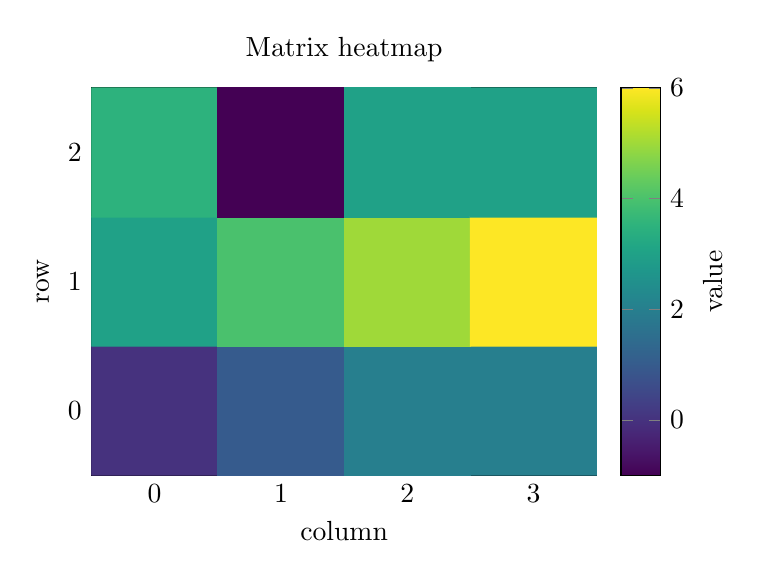
\begin{tikzpicture}
\begin{axis}[
  width=8cm,
  height=6.5cm,
  title={Matrix heatmap},
  title style={align=left},
  colormap/viridis,
  colorbar,
  colorbar style={ylabel={value}},
  xlabel={column},
  xmin=-0.5,
  xmax=3.5,
  xtick={0,1,2,3},
  ylabel={row},
  ymin=-0.5,
  ymax=2.5,
  ytick={0,1,2},
  legend style={draw=none,fill=none,cells={anchor=west}},
]
\addplot+ [mark=none,matrix plot*,point meta=explicit,mesh/rows=3,mesh/cols=4] coordinates {(0,0) [0] (1,0) [1] (2,0) [2] (3,0) [2] (0,1) [3] (1,1) [4] (2,1) [5] (3,1) [6] (0,2) [3.5] (1,2) [-1] (2,2) [2.99] (3,2) [3]};
\end{axis}
\end{tikzpicture}
\end{document}
